% -------------- SCHEMA CONCETTUALE E/R -----------------------------------------

\newpage

\section{Progettazione Concettuale}

\subsection{Schema Scheletro}

\textsf{\small Verranno qui, ora introdotti gli schemi parziali, prendendo in considerazione 4 entità principali, ovvero: }
\begin{enumerate}
	\item \textbf{Passeggero}
	\item \textbf{Compagnia Aerea}
	\item \textbf{Controllore}
	\item \textbf{Volo}
\end{enumerate}

\textsf{\small Dopodichè verranno introdotte le rifinutere e infine lo schema concettuale finale.}\\ % verranno introdotte le rifinutere

% -------------- SCHEMA CONCETTUALE PASSEGGERO ----------------------------------

\enlargethispage{1\linewidth}

\subsubsection{Passeggero}

\textsf{\small Questo schema parziale volge intorno all'entità \textbf{PASSEGGERO} e le sue relazioni con il mondo esterno.}\\ % volge intorno alla figura del

\textsf{\small Il \textbf{passeggero}, gli \textbf{Addetti di scalo}, \textbf{addetti alla sicurezza}, \textbf{aiutanti per disabili} sono una generalizzazione di una entità \textbf{persona}, identificata tramite \emph{codice fiscale}.}\\ %\break

\begin{figure}[H] 
	\centering
	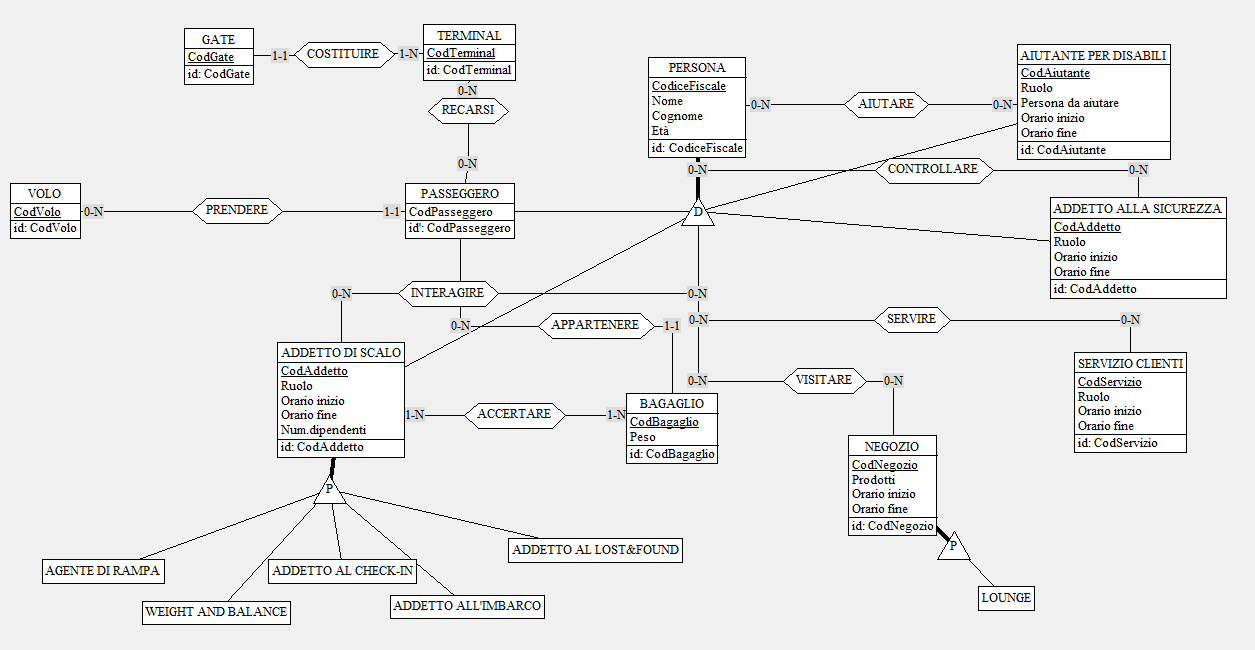
\includegraphics[width=1.2\textwidth, height=1.2\textheight, keepaspectratio]{./img/Schema_Concettuale/Passeggero.png}
	\caption{Schema concettuale di un Passeggero.}
	\label{fig:schema_passeggero}
\end{figure}

\pagebreak

\textsf{Un \textbf{passeggero} che è una figura centrale per il funzionamento di un Aeroporto, può avere diverse relazioni con le \textbf{persone} che lavorano al suo interno:}\\
%che è una figura importante per il funzionamento di un Aeroporto, può avere diverse relazioni con le varie \textbf{persone} che lavorano al suo interno.}

% qui prima era senza lista.
\begin{itemize}
	\item \textsf{\small \emph{Può essere controllato} dagli \textbf{addetti di scalo}, quali \textbf{addetti alla sicurezza} e \textbf{addetti al check-in} .}\\
	\item \textsf{\small \emph{Può visitare} i \textbf{negozi} e le \textbf{lounge} delle \textbf{compagnie aeree}}.\\
	\item \textsf{\small \emph{Può recarsi} al \textbf{servizio clienti} per ottenere informazioni e comprare i biglietti.}\\
	\item \textsf{\small \emph{Può}, una volta comprato un biglietto e superato i controlli \emph{recarsi} al \textbf{terminal} per poi giungere al \textbf{gate} per imbarcarsi e prendere un \textbf{volo}.}\\
\end{itemize}

%\textsf{\small Il \textbf{passeggero} , gli \textbf{Addetti di scalo}, \textbf{addetti alla sicurezza}, \textbf{aiutanti per disabili} sono una generalizzazione di una entità \textbf{persona}. }

% -------------- SCHEMA CONCETTUALE COMPAGNIA AEREA -----------------------------

\newpage

\subsubsection{Compagnia Aerea}

\textsf{\small Dopo aver analizzato il dominio, i problemi e le richieste della Compagnia Aerea, viene qui mostrato il suo schema parziale:}

\begin{figure}[H] 
	\centering
	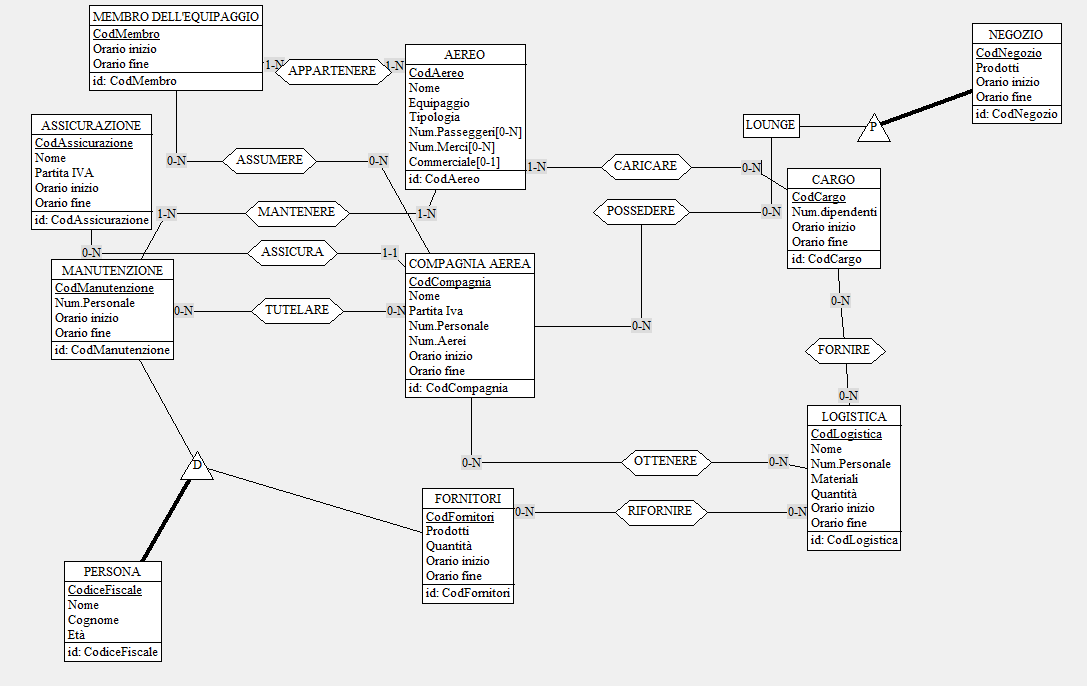
\includegraphics[width=1.2\linewidth, height=1.2\textheight, keepaspectratio]{./img/Schema_Concettuale/Compagnia_Aerea.png}
	\caption{Schema E/R della Compagnia Aerea.}
	\label{fig:schema_compagnia_aerea}
\end{figure}

\textsf{\small Le entità \textbf{Fornitori}, \textbf{Manutentori} e \textbf{Membro dell'equipaggio} rappresentano una estensione più generica di una entità \textbf{Persona}.  }\\

\textsf{\small Una \textbf{compagnia aerea} possiede diversi costi, uno dei primi è in gergo aeronautico \emph{ACMI}, ovvero \emph{Aircraft, Crew, Maintanance, Insurance} (in italiano: \textbf{Aereo}, \textbf{Equipaggio},\textbf{Manutenzione},\textbf{Assicurazione}).}\\

\textsf{\small Inoltre la Compagnia deve rifornire attraverso la \textbf{Logistica} ed il \textbf{Cargo} gli Aerei di beni necessari per il corretto funzionamento del Volo, come carburante, catering, cibo e bevande,ecc..}\\

% -------------- SCHEMA CONCETTUALE CONTROLLORE -----------------------------

\newpage

\enlargethispage{1\linewidth}

\subsubsection{Controllore}

\textsf{\small Figura centrale nella coordinazione e la sicurezza di navigazione degli aeromobili sono i \textbf{Controllori}: }\\
\begin{itemize}
	\item \textbf{\small Di Torre}
	\item \textbf{\small Di Avvicinamento}
	\item \textbf{\small D'Aerea}
\end{itemize}

\textsf{\small questi, rappresentano una estensione più generica di una entità \textbf{Persona}.}\\

\begin{figure}[H] 
	\centering
	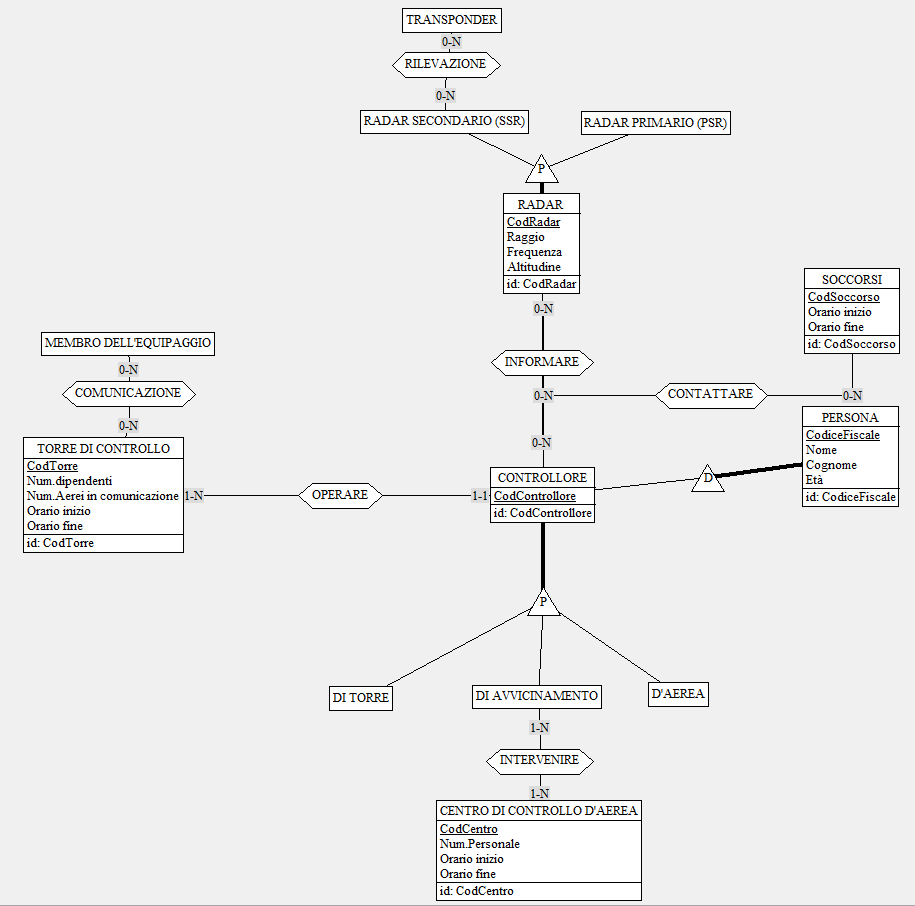
\includegraphics[width=1.2\linewidth, height=1.2\textheight, keepaspectratio]{./img/Schema_Concettuale/Controllore.png}
	\caption{Schema E/R di un Controllore del traffico aereo.}
	\label{fig:schema_controllore}
\end{figure}

\pagebreak

\textsf{\small I \textbf{Controllori}, nella \textbf{Torre di Controllo} o in un \textbf{Centro di Controllo d'Aerea}, attraverso l'utilizzo di uno strumento avanzato di localizzazione chiamato \textbf{Radar} comunicano, organizzano, coordinano il traffico aereo.}\break

% Questa parte è più tecnica che riguardante l'E/R, forse è meglio metterla
% nella parte di analisi/intervista.
\textsf{\small I \textbf{controllori} hanno a che fare con due principali tipi di radar, il PSR (\emph{Primary Surveillance Radar}), \textbf{radar primario di sorveglianza} che \emph{rileva} la posizione di un aeromobile analizzando i segnali che, precedentemente emessi dall'antenna, sono ritornati indietro riflessi dall'obiettivo; dopodichè la posizione dell'aereo può essere letta dall'operatore attraverso uno schermo su cui viene mostrata come una traccia luminosa.}\\

\textsf{\small E il SSR (\emph{Secondary Surveillance Radar}), \textbf{radar secondario di sorveglianza} che a differenza del primario, \emph{rileva} la posizione di un aeromobile analizzando il segnale trasmesso da un apparato a bordo dell'aeromobile (\emph{transponder}), emesso come risposta all'interrogazione ricevuta dal \textbf{radar} a terra.}\break

\textsf{\small In caso di emergenze (\emph{Mayday}), sono pronti a \emph{contattare} i \textbf{soccorsi} che dovranno prestare un tempestivo intervento per garantire la sicurezza dei passeggeri a bordo e del personale aeroportuale a terra. }\\

% -------------- SCHEMA CONCETTUALE VOLO -----------------------------

\newpage

\subsubsection{Volo}

%\textsf{\small Il \textbf{Volo}, l'origine per cui nasce l'Aeroporto, per la navigazione degli aeromobili è qui mostrato in questo ultimo schema parziale.}\\

\textsf{\small Esso congiunge il mezzo, l'\textbf{Aereo} e coloro che debbono usufruire del servizio, i \textbf{Passeggeri}.}\\

\begin{figure}[H] 
	\centering
	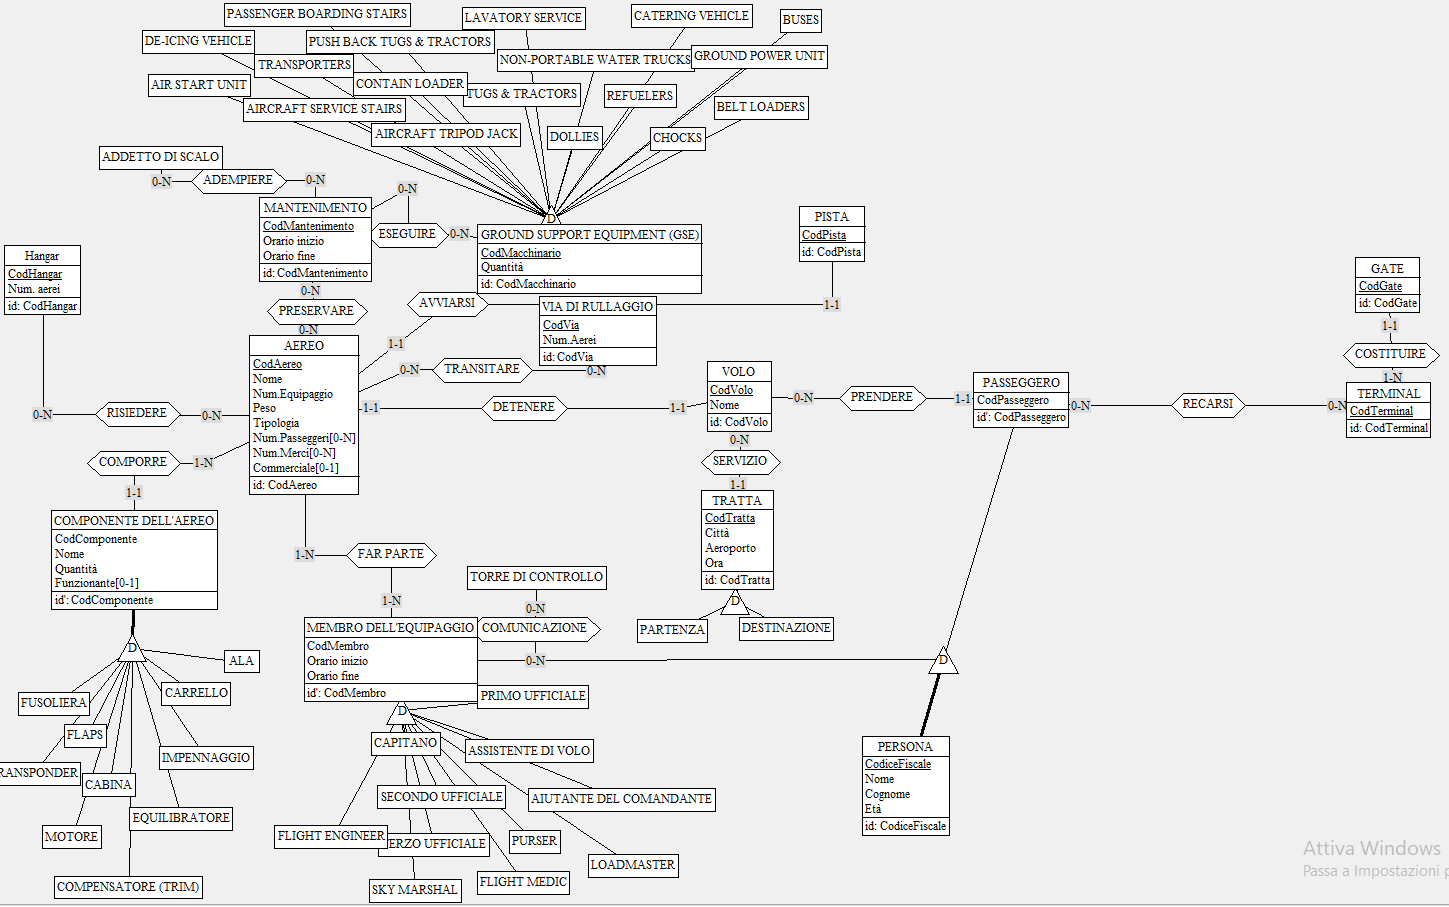
\includegraphics[width=1.2\linewidth, height=1.2\textheight, keepaspectratio]{./img/Schema_Concettuale/Volo.png}
	\caption{Schema E/R del Volo.}
	\label{fig:schema_volo}
\end{figure}

\textsf{\small Un \textbf{Volo} è formato da una \textbf{Tratta} ed un \textbf{Orario}.}\\

\textsf{\small Inoltre, un \textbf{Volo} deve mantenere il contatto radio con la \textbf{Torre di Controllo} per il coordinamento del traffico aereo.}\\

\textsf{\small Ogni \textbf{Aereo} è composto da questi principali componenti:}

\begin{itemize}
	\item \textbf{\small Fusoliera}
	\item \textbf{\small Flaps}
	\item \textbf{\small Ala}
	\item \textbf{\small Carrello}
	\item \textbf{\small Impennaggio}
	\item \textbf{\small Equilibratore}
	\item \textbf{\small Cabina}
	\item \textbf{\small Motore}
	\item \textbf{\small Transponder}
	\item \textbf{\small Compensatore (Trim)}
\end{itemize}

\textsf{\small ed è formato da questi membri dell'equipaggio:}

\textsf{\small \emph{Capitano, Primo Ufficiale, Secondo Ufficiale, Terzo Ufficiale, Flight Engineer, Sky Marshal, Flight Medic, Aiutante del Comandante, Assistente di Volo, Purser, Loadmaster}.} \break

\textsf{\small Di vitale importanza per lo svolgimento in sicurezza delle normali operazioni aeronautiche è la \textbf{Manutenzione}, sia degli \textbf{Addetti di scalo} sia del \textbf{Ground Support Equipment (GSE)}.}\\

\textsf{\small Il \textbf{GSE} è composto da: }\\

\textsf{\small \emph{ Dollies, Chocks, Aircraft Tripod Jack, Aircraft Service Stairs, Refuelers, Tugs and Tractors, Ground Power Unit, Buses, Contain Loader, Transporters, Air Start Unit, Non-portable Water Trucks, Lavatory Service Vehicles, Pushback tugs and tractors, De/anti-Icing Vehicle, Catering Vehicle, Belt Loaders, Passenger Boarding Steps, Aircraft Rescue and Firefighting}.}\\

% -------------- SCHEMA CONCETTUALE FINALE---------------------------------------

%\enlargethispage{1\linewidth}

\subsection{Schema concettuale finale}

\textsf{\small Dati i quattro schemi parziali inziali, presento ora lo \textbf{Schema Concettuale Finale}:}\\

% landscape


%\newgeometry{left = .9mm, right = .9mm, top = .9mm, bottom = .9mm} %TODO: o .6 o .9, top = .6, bottom = .6

\begin{comment}
\begin{sidewaysfigure}[H]
	\includegraphics[width=1.2\textwidth]{./img/Schema_Finale1.png} %TODO: 1 o 1.1 o 1.2, con 1.2 perdiamo delle informazioni, ma si vedo meglio
	\caption{}
	\label{fig:s1}
\end{sidewaysfigure}


\begin{sidewaysfigure}[H]
	\includegraphics[width=1.2\textwidth]{./img/Schema_Finale2.png}
	\caption{}
	\label{fig:s2}
\end{sidewaysfigure}

\begin{sidewaysfigure}[H]
	\includegraphics[width=1.2\textwidth]{./img/Schema_Finale3.png}
	\caption{}
	\label{fig:s3}
\end{sidewaysfigure}

\begin{sidewaysfigure}[H]
	\includegraphics[width=1.2\textwidth]{./img/Schema_Finale4.png}
	\caption{}
	\label{fig:s4}
\end{sidewaysfigure}
\end{comment}

%\restoregeometry

\begin{comment}
\begin{landscape}
	\begin{figure}[H]
		\centering
		\includegraphics[width=1.2\linewidth, height=1.2\textheight, keepaspectratio]{./img/Schema_Finale1.png}
		\caption{Schema concettuale Finale.}
		\label{fig:schema_finale}
	\end{figure}
\end{landscape}
\end{comment}

%TODO: sistemare
\newgeometry{left = .6cm, right = .6cm, top=.1cm, bottom=.1cm} % prima top = 5mm, bottom = 10mm

\begin{figure}[H] 
	\centering
	\includegraphics[width=1.2\linewidth, height=1.2\textheight, keepaspectratio]{./img/Schema_Concettuale/Schema_Finale1.png} 
	\caption{Schema concettuale Finale.}
	\label{fig:schema_finale1}
\end{figure}

\begin{figure}[H] 
	\centering
	\includegraphics[width=1.2\linewidth, height=1.2\textheight, keepaspectratio]{./img/Schema_Concettuale/Schema_Finale2.png}
	\caption{Schema concettuale Finale.}
	\label{fig:schema_finale2}
\end{figure}

\begin{figure}[H] 
	\centering
	\includegraphics[width=1.2\linewidth, height=1.2\textheight, keepaspectratio]{./img/Schema_Concettuale/Schema_Finale3.png}
	\caption{Schema concettuale Finale.}
	\label{fig:schema_finale3}
\end{figure}

\begin{figure}[H] 
	\centering
	\includegraphics[width=1.2\linewidth, height=1.2\textheight, keepaspectratio]{./img/Schema_Concettuale/Schema_Finale4.png}
	\caption{Schema concettuale Finale.}
	\label{fig:schema_finale4}
\end{figure}

\restoregeometry

\begin{comment}
\begin{landscape}
	\begin{figure}[H] %TODO: sistemare grandezza
		\centering
		\includegraphics[width=1\linewidth, height=1\textheight, keepaspectratio]{./img/Schema_Finale1.png} %TODO: o 1 o 1.3 o 1.2
		\caption{Schema concettuale Finale.}
		\label{fig:schema_finale44}
	\end{figure}
\end{landscape}
\end{comment}